\documentclass[11pt,a4paper]{article}
\usepackage{graphicx}
\usepackage{tcolorbox}
\usepackage{xcolor}
\usepackage{geometry}
\usepackage{tikz}
\geometry{margin=0.8in}

% Define colors
\definecolor{mlblue}{RGB}{31, 119, 180}
\definecolor{mlorange}{RGB}{255, 127, 14}
\definecolor{mlgreen}{RGB}{44, 160, 44}
\definecolor{mlred}{RGB}{214, 39, 40}
\definecolor{mlpurple}{RGB}{148, 103, 189}

\title{\Large\textbf{Discovery 2: The Feature Detective}\\
\vspace{0.3em}
\normalsize Same Data, Different Stories}
\date{}

\begin{document}
\maketitle
\vspace{-2em}

\section*{One Dataset, Three Views}

\begin{center}
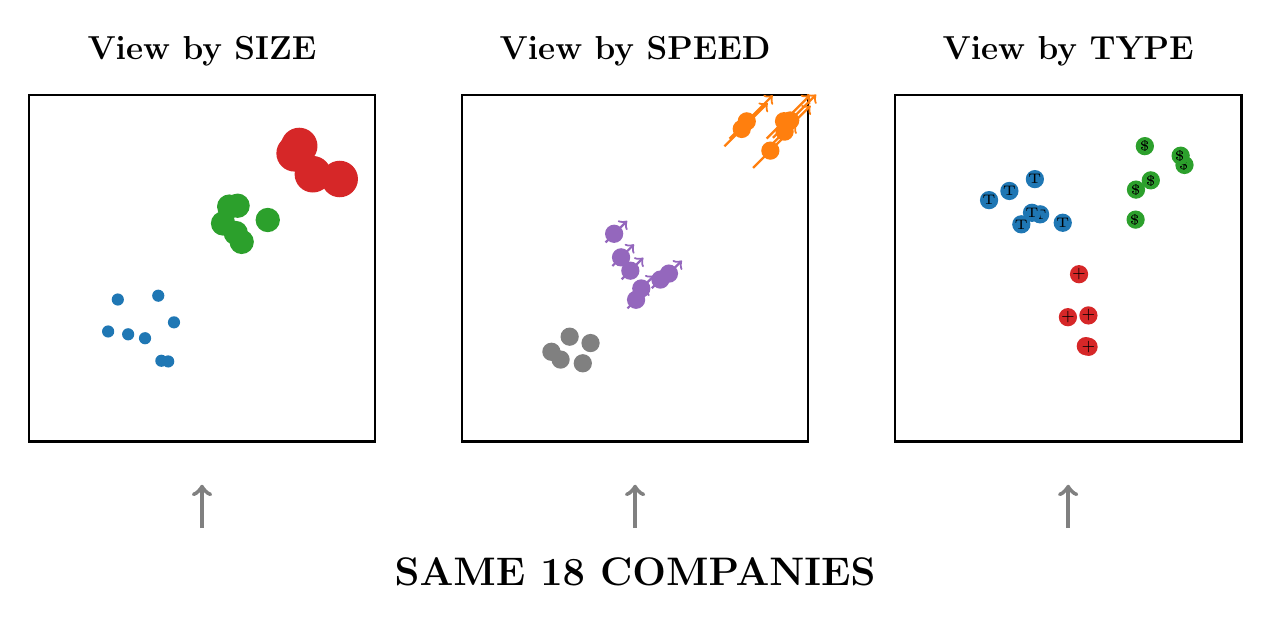
\begin{tikzpicture}[scale=1.1]
% View 1: By Size
\begin{scope}[shift={(0,0)}]
\draw[thick] (-1,-1) rectangle (3,3);
\node[font=\large] at (1,3.5) {\textbf{View by SIZE}};
% Small companies cluster
\foreach \i in {1,...,8} {
    \pgfmathsetmacro{\x}{0.3 + rand*0.4}
    \pgfmathsetmacro{\y}{0.3 + rand*0.4}
    \fill[mlblue] (\x,\y) circle (2pt);
}
% Medium companies
\foreach \i in {1,...,6} {
    \pgfmathsetmacro{\x}{1.5 + rand*0.3}
    \pgfmathsetmacro{\y}{1.5 + rand*0.3}
    \fill[mlgreen] (\x,\y) circle (4pt);
}
% Large companies
\foreach \i in {1,...,4} {
    \pgfmathsetmacro{\x}{2.3 + rand*0.3}
    \pgfmathsetmacro{\y}{2.3 + rand*0.3}
    \fill[mlred] (\x,\y) circle (6pt);
}
\end{scope}

% View 2: By Speed
\begin{scope}[shift={(5,0)}]
\draw[thick] (-1,-1) rectangle (3,3);
\node[font=\large] at (1,3.5) {\textbf{View by SPEED}};
% Same data, different grouping
\foreach \i in {1,...,6} {
    \pgfmathsetmacro{\x}{2.5 + rand*0.3}
    \pgfmathsetmacro{\y}{2.5 + rand*0.3}
    \fill[mlorange] (\x,\y) circle (3pt);
    \draw[->, thick, mlorange] (\x-0.2,\y-0.2) -- (\x+0.3,\y+0.3);
}
\foreach \i in {1,...,7} {
    \pgfmathsetmacro{\x}{1 + rand*0.4}
    \pgfmathsetmacro{\y}{1 + rand*0.4}
    \fill[mlpurple] (\x,\y) circle (3pt);
    \draw[->, thick, mlpurple] (\x-0.1,\y-0.1) -- (\x+0.15,\y+0.15);
}
\foreach \i in {1,...,5} {
    \pgfmathsetmacro{\x}{0.2 + rand*0.3}
    \pgfmathsetmacro{\y}{0.2 + rand*0.3}
    \fill[gray] (\x,\y) circle (3pt);
}
\end{scope}

% View 3: By Industry
\begin{scope}[shift={(10,0)}]
\draw[thick] (-1,-1) rectangle (3,3);
\node[font=\large] at (1,3.5) {\textbf{View by TYPE}};
% Tech cluster
\foreach \i in {1,...,7} {
    \pgfmathsetmacro{\x}{0.5 + rand*0.5}
    \pgfmathsetmacro{\y}{2 + rand*0.5}
    \fill[mlblue] (\x,\y) circle (3pt);
    \node[font=\tiny] at (\x,\y) {T};
}
% Finance cluster
\foreach \i in {1,...,6} {
    \pgfmathsetmacro{\x}{2 + rand*0.5}
    \pgfmathsetmacro{\y}{2 + rand*0.5}
    \fill[mlgreen] (\x,\y) circle (3pt);
    \node[font=\tiny] at (\x,\y) {\$};
}
% Health cluster
\foreach \i in {1,...,5} {
    \pgfmathsetmacro{\x}{1 + rand*0.5}
    \pgfmathsetmacro{\y}{0.5 + rand*0.5}
    \fill[mlred] (\x,\y) circle (3pt);
    \node[font=\tiny] at (\x,\y) {+};
}
\end{scope}

% Arrows showing same data
\draw[->, ultra thick, gray] (1,-2) -- (1,-1.5);
\draw[->, ultra thick, gray] (6,-2) -- (6,-1.5);
\draw[->, ultra thick, gray] (11,-2) -- (11,-1.5);
\node at (6,-2.5) {\Large\textbf{SAME 18 COMPANIES}};
\end{tikzpicture}
\end{center}

\vspace{1em}

\begin{tcolorbox}[colback=mlorange!10, colframe=mlorange!50]
\centering\Large
\textbf{Which view tells the truth?}
\end{tcolorbox}

\vspace{2em}

\section*{The Curse of Too Many Features}

\begin{center}
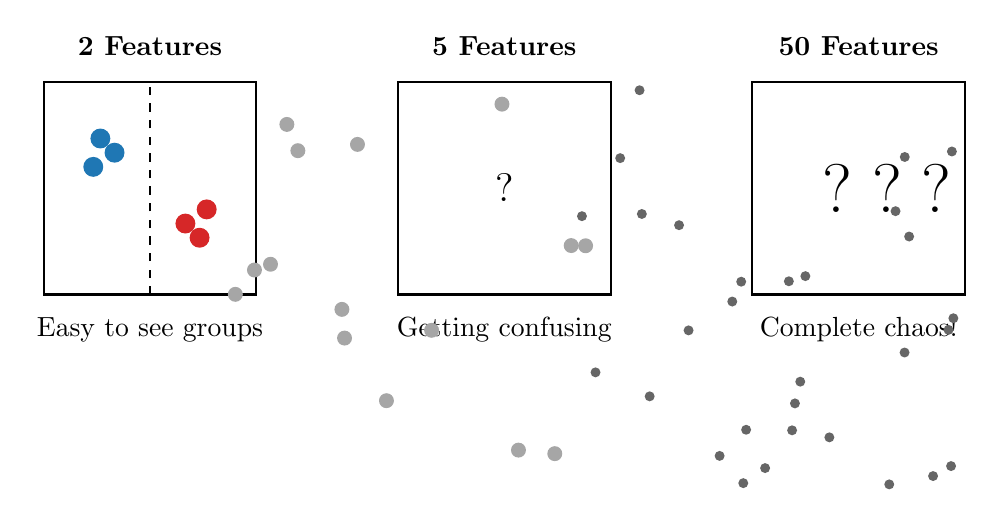
\begin{tikzpicture}[scale=0.9]
% 2D space - clear separation
\draw[thick] (0,0) rectangle (3,3);
\node at (1.5,3.5) {\textbf{2 Features}};
\node at (1.5,-0.5) {Easy to see groups};
\fill[mlblue] (0.8,2.2) circle (4pt);
\fill[mlblue] (1,2) circle (4pt);
\fill[mlblue] (0.7,1.8) circle (4pt);
\fill[mlred] (2.2,0.8) circle (4pt);
\fill[mlred] (2,1) circle (4pt);
\fill[mlred] (2.3,1.2) circle (4pt);
\draw[dashed, thick] (1.5,0) -- (1.5,3);

% 5D space - getting confused
\draw[thick] (5,0) rectangle (8,3);
\node at (6.5,3.5) {\textbf{5 Features}};
\node at (6.5,-0.5) {Getting confusing};
\foreach \i in {1,...,15} {
    \pgfmathsetmacro{\x}{5.2 + rand*2.6}
    \pgfmathsetmacro{\y}{0.2 + rand*2.6}
    \fill[gray!70] (\x,\y) circle (3pt);
}
\node[font=\Large] at (6.5,1.5) {?};

% 50D space - chaos
\draw[thick] (10,0) rectangle (13,3);
\node at (11.5,3.5) {\textbf{50 Features}};
\node at (11.5,-0.5) {Complete chaos!};
\foreach \i in {1,...,30} {
    \pgfmathsetmacro{\x}{10.1 + rand*2.8}
    \pgfmathsetmacro{\y}{0.1 + rand*2.8}
    \fill[black!60] (\x,\y) circle (2pt);
}
\foreach \i in {1,...,3} {
    \node[font=\Huge] at (10.5+\i*0.7,1.5) {?};
}
\end{tikzpicture}
\end{center}

\newpage

\section*{Your Turn: Feature Hunt}

\begin{center}
\Large
Pick something you know well (your class, favorite apps, local restaurants...)

\vspace{2em}

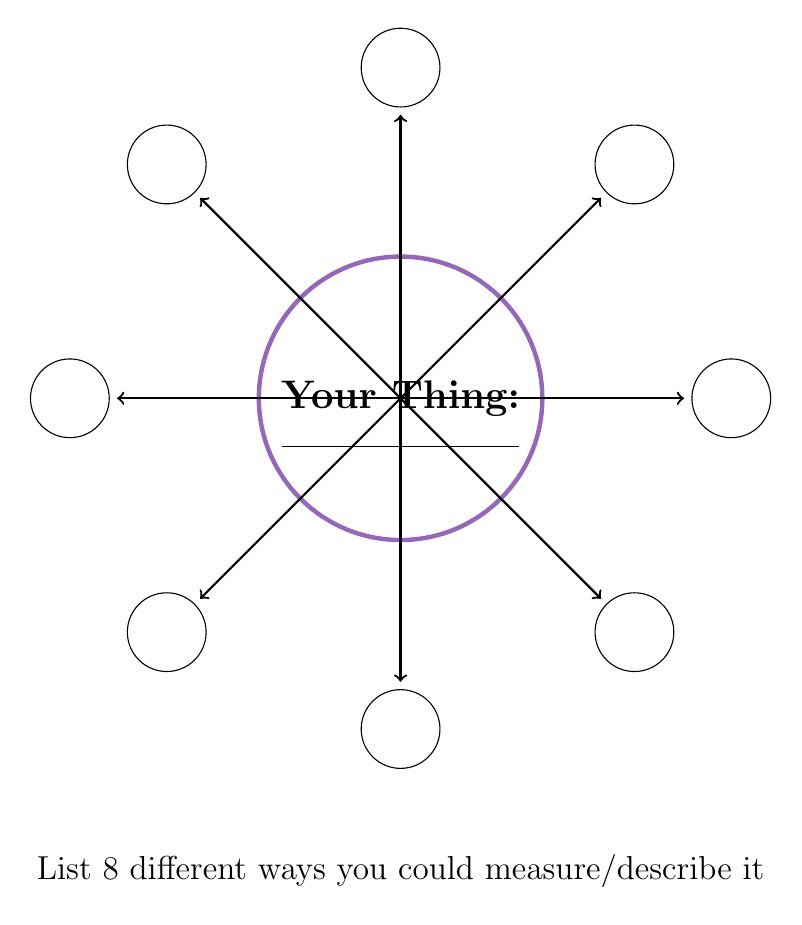
\begin{tikzpicture}[scale=1.2]
% Central item
\draw[ultra thick, mlpurple] (0,0) circle (1.5);
\node at (0,0) {\Large\textbf{Your Thing:}};
\node at (0,-0.5) {\underline{\hspace{3cm}}};

% Feature spokes
\foreach \angle/\label in {0/Feature 1, 45/Feature 2, 90/Feature 3, 135/Feature 4, 180/Feature 5, 225/Feature 6, 270/Feature 7, 315/Feature 8} {
    \draw[->, thick] (0,0) -- (\angle:3);
    \node[draw, circle, minimum size=1cm] at (\angle:3.5) {};
}

\node at (0,-5) {\large List 8 different ways you could measure/describe it};
\end{tikzpicture}

\vspace{2em}

Now pick your TOP 2 features:

\vspace{1em}
\textbf{Feature A:} \underline{\hspace{5cm}} \textbf{Feature B:} \underline{\hspace{5cm}}

\vspace{2em}

Draw how things would group using ONLY these 2:

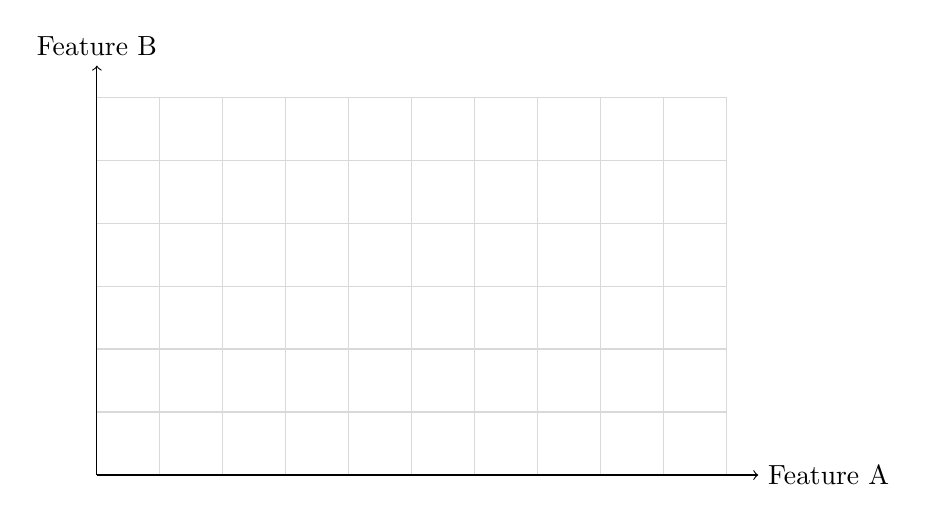
\begin{tikzpicture}[scale=0.8]
\draw[gray!30] (0,0) grid (10,6);
\draw[->] (0,0) -- (10.5,0) node[right] {Feature A};
\draw[->] (0,0) -- (0,6.5) node[above] {Feature B};
\end{tikzpicture}
\end{center}

\vspace{1em}

\begin{tcolorbox}[colback=mlpurple!10, colframe=mlpurple!50]
\centering\large
\textbf{Next Class:} How ML handles 100+ features at once
\end{tcolorbox}

\end{document}